\documentclass{report}
\usepackage{graphicx}
\usepackage{float}
\usepackage{amsmath}
\usepackage{amsthm}
\usepackage{caption}
\usepackage{algorithm}
\usepackage{hyperref}
\usepackage[noend]{algpseudocode}

\renewcommand{\algorithmicrequire}{\textbf{input:}}
\renewcommand{\algorithmicensure}{\textbf{output:}}

\usepackage{mathtools}
\declarepaireddelimiter\ceil{\lceil}{\rceil}

\def \scalingfactor{.8}

\begin{document}

\title{insert appropriate title here}
\author{cl\'{e}ment humbert, tristan overney\and paolo ienne, andrea miele, ewaida mohsen (supervisors)}
\date{\today}
\maketitle

\nocite{*}

\setcounter{tocdepth}{1}
\tableofcontents
\listoffigures

\chapter{introduction}

    due to their simd nature, gpus have been used in different scientific fields to perform
    non-graphical computations for a while. they're used for particle and molecular dynamic 
    modeling, astrophysic and fluid mechanic modeling.
    more recently they've been used for cryptographic applications and in particular
    to factorize large numbers in an attempt to compromise rsa encryption \cite{cofact14}.
    cryptography-related applications make heavy use of very large integer operations.
    here's an algorithm as example from \cite{cofact14}:
    \begin{algorithm}
    \caption{Large operands multiplication}\label{alg:mulalgo}
    \begin{algorithmic}[1]
        \require{integers x and $y=\sum_{i=0}^{n-1}y_ir^i$ such that $0\leq x$, $y_i<r$ for $0\leq i<n$.}
        \ensure{$z=x\cdot y = \sum_{i=0}^nz_ir^i$}
        \state mul.lo($z_0$, x, $y_0$)
        \state mul.hi($z_1$, x, $y_0$)
        \state mad.lo.cc($z_1$, x, $y_1$, $z_1$)
        \state mul.hi($z_2$, x, $y_1$)
        \for{$i=2$ to $n-2$}
            \state madc.lo.cc($z_i$, x, $y_i$, $z_i$)
            \state mul.hi($z_{i+1}$, x, $y_i$)
        \endfor
        \state madc.lo.cc($z_{n-1}$, x, $y_{n-1}$, $z_{n-1}$)
        \state madc.hi($z_n$, x, $y_{n-1}$, 0)
        \state \textbf{return} $z (=\sum_{i=0}^nz_ir^i)$
    \end{algorithmic}
    \end{algorithm}

    Due to the nature of asymmetric cryptography, these applications are bound by
    integer computing capacity which is not the focus of GPU. GPUs are designed
    around floating-point number operations, for older GPUs it was single-precision
    floating-point number (which will be referred to as float from now on) operations and
    on more recent GPUs tendency is to focus on double precision floating-point number operations.
    Fermi generation is the last generation to have decent integer multiplication performances
    compared to its float performance. It is one of the reason it was chosen for this project.

\section{goals}
    the aim of this project is to study and identify the limitations of gpus
    when used for cryptography and large integers computation in order to suggest
    hardware changes with integer capabilities appropriate for integer-heavy applications.

\chapter{first approach}
    the first idea to enhance the cryptographic capabilities of the gpu is to
    build crypto specific hardware into the original hardware to expose new 
    operations (in the form of assembly opcodes) to the developers with the 
    shortest latency possible. 
    
    an algorithm that is constantly used in cryptography is the montgomery multiplication,
    a special kind of modular multplication. implementing such an operation in hardware can
    be done in many ways, one of the most efficient is the rolled implementation described
    by the algorithm \ref{alg:montgomery}. Where operands $X$ and $Y$ would have been prepared
    by software for the multiplication And that can be unrolled for the hardware implementation
    in order to allow for pipelining.
    
    \begin{algorithm}
    \caption{Hardware Montgomery multiplier\cite{montgomeryHard}}\label{alg:montgomery}
    \begin{algorithmic}[1]
        \require{integers $x$, $y$ and $m$ with $0\leq x$, $y < m$.}
        \ensure{$p=(x * y (2^n)^{-1})\text{ mod }m$.}
        \statex $n$ is the number of bits in $x$.
        \statex $x_i$ is the $i^{th}$ bit of $x$.
        \statex $s_0$ is the least significant bit of $s$. 		
        \state $s := 0$; $c := 0$; \comment $s$ is the sum and $c$ is the carry
        \for{$i=0$; $i < n$; $i++$}
            \state $s,c := s + c + x_i * y$; \comment $s,c := ...$ is a carry-save adder assignation
            \state $s,c := s + c + s_0 * m$;
            \state $s := s$ div $2$; $c := c$ div $2$;  
        \endfor
        \state $p := s + c$;
        \if{ $p \geq m$}
            \state $p := p - m$;
        \endif
        \state \textbf{return} $p$;
    \end{algorithmic}
    \end{algorithm}
    
    other ways to do the cryptography enhancement would be to have part of such
    an algorithm implemented in hardware and the rest in software.
    such as multiplications of numbers larger than 32bits.
    

    the impact of the new opcodes were to be measured with the assistance of
    gpgpu-sim\cite{gpgpusim09} a fermi architecture simulator. it was determined
    that new opcodes can be added to gpgpu-sim and included in an instruction group
    to modify its latency (an unused operation could have been chosen to set the new
    instruction's latency).

    to determine the speed/size of the new components the original cores have to
    be studied as not much is known from nvidia sources. in order to understand 
    the cores and be able to suggest meaningful changes, a serie of microbenchmarking 
    experiments had to be done. 


\chapter{fermi's architecture}
    before diving into the experiments and their results here's a quick-start
    guide to nvidia's fermi architecture and its vocabulary:
    \section{streaming multiprocessors}
    the largest building block inside the fermi architecture is the 
    \emph{streaming multiprocessor} (figure ~\ref{fig:sm} on page 
    ~\pageref{fig:sm}) abbreviated sm in this report. the gtx580 card is equipped
    with 16 of these sms.
    \begin{figure}[h]
    \centering
        \includegraphics[width=0.75\linewidth]{pictures/fermi}
        \captionsetup{justification=centering}
        \caption{Fermi's SM schematic representation.\cite{fermiwhitepap}}
        \label{fig:SM}
    \end{figure}

    each sm is composed of the following computation blocks\cite{fermiwhitepap}:
    \begin{itemize}
        \item 32 cuda cores in two groups of 16,
        \item 16 load/store units (ld/st on the figure)
        \item 4 special functions units (sfus) dedicated to more complex
              arithmetic functions such as sines and logarithms.
    \end{itemize}
    
    As the SFU is dedicated to complex float operations it's already an area
    that can be reused for integer computation components, thus it's not part
    of the following research. The focus of the experiments are the CUDA cores.
    
    Integer is supported with at most 32-bits in Fermi.

    \section{cuda cores}
    figure~\ref{fig:cudacore} is the representation of what a cuda core is,
    according to nvidia\cite{fermiwhitepap}.
    
    \begin{figure}[h]
    \centering
        \includegraphics[width=0.5\linewidth]{pictures/cudacore}
        \captionsetup{justification=centering}
        \caption{schematic representation of nvidia's cuda core.}
        \label{fig:cudacore}
    \end{figure}
    
    From figure~\ref{fig:CUDACore} the notion of twice 16 cores can be
    adjusted to 2x16 integers ALUs and 2x16 float ALUs.

    \section{Basics of Fermi's scheduling}
        \subsection{Grids and blocks} 
        A cuda kernel (that is: a section of code that will run on the GPU) is
        launched with two parameters: a grid size and a block size. The grid 
        size is used to determine the number of SM on which the code will run.
        The block size determines how many threads will run the code inside each
        SM\cite{cudaprog}. As we're interested in the properties of single SMs or even, single
        cores, every benchmarking experiment was done using a grid size of one.

        \subsection{warps}
        the second important scheduling unit is the warp. a warp consists
        of 32 threads. each scheduling cycle, the scheduler selects two
        warps, for each of these it schedules 16 threads (making it 32
        threads scheduled, coming from two warps)\cite{cudaprog}.

\chapter{benchmarking}

\section{methods}
	to get informations about the microarchitecture of the cuda cores, a serie 
    of specially crafted cuda kernels were used. these usually contain large 
    batches of instructions that were timed with the assistance of the \texttt{clock64()} 
    function offered by the cuda api.

	the benchmark programs have been ran on a machine equipped with an nvidia
    geforce gtx 580 gpu used by \cite{cofact14}.

\section{pipeline properties}
	this section contains the results obtained through the previously described
	methods using large batches of integer multiplications.

	\subsection{benchmark running times against number of threads}
	\label{par:pipeline_exp}
	\subsubsection{description of the experiment}
	the first experiment aims at outlining the relation between the running
    times of the benchmark program and the number of threads running parallely in
    a single block (the threads reside on one SM).
	\subsubsection{Expectations}
    The running times are expected to be slightly higher for the integer
    multiplications, as GPUs are optimized for float computation
    but to deteriorate in a similar fashion (begin to deteriorate
    at the same point, at the same rate) due to each core being equipped with
    integer and float ALUs.
    
	\subsubsection{results and analysis}
    \begin{figure}[h]
    	\centering
		\vspace{-20pt}
	    \includegraphics[width=\scalingfactor\linewidth]{"graphics/float_vs_int_running_times"}
		\vspace{-15pt}
		\captionsetup{justification=centering}
        \caption{running times of benchmark (in cycles) against number of threads.}
    \end{figure}
	
    the results are against the expectations as it's easy to see the integer
    multiplication times starting to grow at 289 threads in the block against
    577 for the float multiplications.
    
    %not at the right place, there should be a section about FP benchmark.
    As the running time is constant up to 576 threads running in parallel and that we have 32 cores
    available, the hypothesis has been formulated that the pipeline depth for the float multiplication is 18 ($576/32 = 18$). Which seems to correlate with the running
    times of the integers multiplication. 
    
    figure~\ref{fig:fp_prediction_512}
    represents the hypothesis made about the pipeline depth when 576 threads are running, $c_1$ to
    $c_{32}$ are the core of the single sm on which the experiment has been run. (1 to 16 is the
    first core group and 17 to 32 is the second one.) $t_{j,k}$ is the $k$-eme instruction of the thread number $j$. 
        \begin{figure}[h]
      \centering
       \begin{tabular}{ | r || c | c | c | c || c | c | c | }
    	    \hline
    	    time since beginning & $c_1$ & $c_2$ & ... & $c_{16}$ & $c_{17}$ & ... & $c_{32}$ \\ \hline  \hline
    	   1 & $t_{0,0}$ & $t_{1,0}$ & ... & $t_{15,0}$ & $t_{32, 0}$ & ... & $t_{47, 0}$ \\ \hline 
    	   2 & $t_{16,0}$ & $t_{17,0}$ & ... & $t_{31,0}$ & $t_{48, 0}$ & ... & $t_{63, 0}$ \\ \hline
    	   3 & $t_{64,0}$ & $t_{65,0}$ & ... & $t_{79,0}$ & $t_{96, 0}$ & ... & $t_{111, 0}$ \\ \hline
    	   ... & ... & ... & ... & ... & ... & ... & ... \\ \hline
    	   16 & $t_{528,0}$ & $t_{529,0}$ & ... & $t_{543,0}$ & $t_{560,0}$ & ... & $t_{575, 0}$ \\ \hline
    	   17 & $t_{0,1}$ & $t_{1,1}$ & ... & $t_{15,1}$ & $t_{32, 1}$ & ... & $t_{47, 1}$ \\ \hline
    	   ... & ... & ... & ... & ... & ... & ... & ... \\ \hline
  	\end{tabular}
  	\captionsetup{justification=centering}
  	\caption{Planned running scheme for 576 threads with float multiplication.}
  	\label{fig:fp_prediction_512}
   \end{figure}
   
    figure~\ref{fig:int_prediction_256} represents the hypothesis made about the pipeline when 288
    threads are running, $c_1$ to $c_{32}$ are the core of the single sm on which the experiment
    has been run. (1 to 16 is the first core group and 17 to 32 is the second one.). the first
    group core is provided in integer multiplication but the second. $t_{j,k}$ is the $k$-eme instruction of the thread number
    $j$.
   \begin{figure}[h]
      \centering
       \begin{tabular}{ | r || c | c | c | c || c | c | c | }
    	    \hline
    	    time since beginning & $c_1$ & $c_2$ & ... & $c_{16}$ & $c_{17}$ & ... & $c_{32}$ \\ \hline  \hline
    	   1 & $t_{0,0}$ & $t_{1,0}$ & ... & $t_{15,0}$ & - & ... & - \\ \hline 
    	   2 & $t_{16,0}$ & $t_{17,0}$ & ... & $t_{31,0}$ & - & ... & - \\ \hline
    	   3 & $t_{32,0}$ & $t_{33,0}$ & ... & $t_{47,0}$ & - & ... & - \\ \hline
    	   ... & ... & ... & ... & ... & ... & ... & ... \\ \hline
    	   18 & $t_{272,0}$ & $t_{273,0}$ & ... & $t_{287,0}$ & - & ... & - \\ \hline
    	   19 & $t_{0,1}$ & $t_{1,1}$ & ... & $t_{15,1}$ & - & ... & - \\ \hline
    	   ... & ... & ... & ... & ... & ... & ... & ... \\ \hline
  	\end{tabular}
  	\captionsetup{justification=centering}
  	\caption{planned running scheme for 288 threads with integer number multiplication.}
  	\label{fig:int_prediction_256}
   \end{figure}

    to understand these deterioration points the next experiment has been designed.

\section{understanding pipeline length and performance deterioration}
    \subsection{the experiment}
    with the results of \ref{par:pipeline_exp} in mind, it's clear that the pipelines depth 
    must be 18. the objective of the following experiment is to determine the cost of
    the loop used in the benchmarks to adjust the running times found and see if they match with
    the hypothesis about pipeline length and scheduling. 
	\subsubsection{Expectations}
	As seen in \ref{par:pipeline_exp} the cost of float
    operations goes up at 576 threads. This would imply that every pipeline of
    the SM is perfectly filled with 576 threads. Dividing 576 threads by
    the 32 cores gives a pipeline length of 18. In addition, the cost increase
    is suspected to be 1/9 of the base cost as the scheduling is expected to be
    something like described in the following schematic:
    
    \begin{figure}[h]
      \centering
       \begin{tabular}{ | r || c | c | c | c || c | c | c | }
    	    \hline
    	    time since beginning & $c_1$ & $c_2$ & ... & $c_{16}$ & $c_{17}$ & ... & $c_{32}$ \\ \hline  \hline
    	   1 & $t_{0,0}$ & $t_{1,0}$ & ... & $t_{15,0}$ & $t_{32, 0}$ & ... & $t_{47, 0}$ \\ \hline 
    	   2 & $t_{16,0}$ & $t_{17,0}$ & ... & $t_{31,0}$ & $t_{48, 0}$ & ... & $t_{63, 0}$ \\ \hline
    	   3 & $t_{64,0}$ & $t_{65,0}$ & ... & $t_{79,0}$ & $t_{96, 0}$ & ... & $t_{111, 0}$ \\ \hline
    	   ... & ... & ... & ... & ... & ... & ... & ... \\ \hline
    	   18 & $t_{528,0}$ & $t_{529,0}$ & ... & $t_{543,0}$ & $t_{560,0}$ & ... & $t_{575, 0}$ \\ \hline
    	   19 & $t_{576,0}$ & - & ... & - & - & ... & - \\ \hline
    	   20 & - & - & ... & - & - & ... & - \\ \hline
    	   21 & $t_{0,1}$ & $t_{1,1}$ & ... & $t_{15,1}$ & $t_{32,1}$ & ... & $t_{47,1}$ \\ \hline
    	   ... & ... & ... & ... & ... & ... & ... & ... \\ \hline
  	\end{tabular}
  	\captionsetup{justification=centering}
  	\caption{Planned running scheme for 577 threads with float multiplication.}
  	\label{fig:fp_prediction_513}
   \end{figure}

    the 1/9 can be derived from the following formula
    \[ \cfrac{t_{\text{577threads}} - t_{\text{576threads}}}{t_{\text{576threads}}} \text{  .}\]
    the latency of an instruction is equal to the pipeline length, plus 1/18 of
    it for every additional warp after the $18^{\text{th}}$. so the latency l of an 
    operation is $l + \text{max}(0, \ceil{\cfrac{n}{32} -18})$ and to get the total
    running time of a benchmark, this latency must be added as a constant to
    represent the time the last instruction takes to get through the pipeline.

    the expansion of the previous formula gives
    \[ \cfrac{(18\cdot l_{576} + l_{577} + l_{577}) - (18\cdot l_{576} + l_{576})}{18\cdot l_{576} + l_{576}} \text{  .}\]
    which, with numerical values and simplifications is
    \[ \cfrac{(18\cdot 19 + 2\cdot 19) - (18^2 + 18)}{18^2 + 18} = \cfrac{1}{9}\text{  .}\] 

    thus, the outcome expected is that once the loop cost is removed from the 
    times obtained in \ref{par:pipeline_exp} the remaining time is 18 millions
    which is 18 cycles per operation, fitting the 18-stages pipeline hypothesis.
    the expected difference in running time after adjustments is 2 millions cycles,
    1/9 of 18 millions.

	\subsubsection{results and analysis}
    \begin{figure}[h]
		\centering
		\vspace{-20pt}
    			\includegraphics[width=\scalingfactor\linewidth]{"graphics/for-sizes-superpositions"}
		\vspace{-15pt}
		\captionsetup{justification=centering}
		\caption{running a million operations broken down in 10 and 1000 loop iterations.}
        \label{fig:for-cost}
	\end{figure}
    
    figure ~\ref{fig:for-cost} suggests that only a insignificant amount of time is spent by the loop
    iterations' instructions. the next possible explanation would be data transfer overhead caused
    by compiler shenanigans.

\section{Mixing float and integer multiplication}
	\subsection{The experiment}
	Information has been found in \ref{par:pipeline_exp} that was implying that the number of 
    integer multiplication able to run parallely on an SM was only half the number of 
    float multiplication. Leading to the conclusion that only one of
    the two 16 cores group of an SM was equipped with integer. The following experiments issue 
    integer multiplication in parallel of float operations to confirm this hypothesis.
	\subsection{Benchmark running times, 1 float multiplication for 1 integer multiplication}
	If indeed only 1 out of 2 cores group can run integer multiplication then
    adding the same amount of float multiplications as there were integer
    multiplications should not increase the total time spent executing the benchmark 
    program as the float multiplication can
    be ran on the other core group (the one that does not possess integer multiplication).
	
	one million multiplication of each kind has been ran on 1 to 1024 threads to
    see if the results were comparable to the graph were there was only integer multiplication.
	%todo update that hideous graph!
	\begin{figure}[h]
		\centering
		\vspace{-20pt}
    			\includegraphics[width=\scalingfactor\linewidth]{"graphics/running_times_ratio11"}
		\vspace{-15pt}
		\captionsetup{justification=centering}
		\caption{Integer/Float multiplication ratio: 1.}
	\end{figure}
	\pagebreak

	\subsection{Benchmark running times with mixed float multiplications and integer multiplications}
	\begin{figure}[H]
		\centering
		\vspace{-20pt}
        \includegraphics[width=\scalingfactor\linewidth]{"graphics/running_times_mixed"}
		\vspace{-15pt}
		\captionsetup{justification=centering}
        \caption{Running times of benchmarks with a mix of flaot multiplications and integers multiplications.}
    \end{figure}

    \subsection{results}
    the running times appear to be bound by those of the integer multiplication but is no higher than
    when only integer multiplications are ran, this confirms the hypothesis that only 16 of the 32
    cuda core are equipped with integer alus. 

\section{Results}
    \subsection{Pipeline structure}
    As seen during the experiments, the CUDA core's pipeline appears to be an
    18 steps pipeline. The fact that integer multiplication and 
    float multiplication both take the same amount
    of time (on a machine that's supposed to be a float computation
    optimized device) until the pipelines are filled suggests a simple,
    no-dependency-check, scheduler that fires up new instructions every 18 cycles.

    it also appears rather clearly that, while 32 cores per sm are advertised by
    nvidia, only 16 are equipped with integer alus; allowing only 18 integer
    operations to be scheduled every 18 cycles.
    
    \subsection{prospects}
    from the previous constatations the following ideas are expected to drastically
    improve the integer computation performances while maintaining a stable (if not
    lower) cost in transistors:
    \begin{itemize}
        \item if any instruction is to be added (e.g.: montgomery's multiplication, larger integer multiplication) these can take up to 18 cycles without having to modify any aspect of the scheduler.
        \item a large amount of integer computation power can be added at low-cost as a whole 16-cores group can be totally replaced by cores dedicated to integer arithmetic.
    \end{itemize}
\section{additional graphics and tables}
	\subsection{integer multiplication: 1024 threads starting times}
    \begin{figure}[h]
    		\centering
		\vspace{-20pt}
	    	\includegraphics[width=\scalingfactor\linewidth]{"graphics/starting_times_ratio31"}
	    	\vspace{-15pt}
	    	\captionsetup{justification=centering}    
	    	\caption{order in which thread batches are started.}
    \end{figure}
\chapter{Beyond the current architecture}
    Given the knowledge acquired with all those experiments. The internal functioning of a Fermi SM was much clearer. And it was now possible to say what could possibly changed and whatnot.
   \section{Proposed enhancement}
   The most obvious upgrade that could be implemented would be to have the two core group to be identical in order to boost the issue rate of integer multiplication to a float multiplication-like performance.
   \begin{figure}[H]
      \centering
       \begin{tabular}{ | c | c | }
    	    \hline
    	    $1^{st}$ cuda core group & $2^{nd}$ cuda core group \\ \hline
    	   float unit and 32-bit multiplier & float unit \\ \hline
  	\end{tabular}
  	\captionsetup{justification=centering}
  	\caption{current cuda core configuration.}
  	\label{fig:current_cores}
   \end{figure}
   There is two distinct approaches to this modification which are described as plan A and plan B in the following part of the report.
   \subsection{Plan A: 32-bit integer multiplier for every core}
    In this first scenario, the change would be to add a 32-bit multiplier to every core that doesn't have one yet. So all 32 cores would have a full float unit and a 32-bit multiplier.
    \begin{figure}[H]
      \centering
       \begin{tabular}{ | c | c | }
    	    \hline
    	    $1^{st}$ cuda core group & $2^{nd}$ cuda core group \\ \hline
    	   float unit and 32-bit multiplier & float unit and 32-bit multiplier \\ \hline
  	\end{tabular}
  	\captionsetup{justification=centering}
  	\caption{first plan cuda core new configuration.}
  	\label{fig:plana_cores}
   \end{figure}
    The expected outcome in term of issue rate would stay the same for float multiplication so 32 per clock cycle per SM. But the integer multiplication issue rate, which is assumed to have become the same as the float multiplication issue rate, is expected to also be 32 per clock cycle per SM.
    The advantage of this plan is that there is far less changes to the existing cores than plan B.
   \subsection{Plan B: Every core with only integer support}
   In this second plan, instead of just adding 32-bit multiplier as in plan A; the change would be to have no more float support but instead have 32 integer only units with 32-bit multiplier.
   \begin{figure}[H]
      \centering
       \begin{tabular}{ | c | c | }
    	    \hline
    	    $1^{st}$ cuda core group & $2^{nd}$ cuda core group \\ \hline
    	   32-bit multiplier & 32-bit multiplier \\ \hline
  	\end{tabular}
  	\captionsetup{justification=centering}
  	\caption{second plan cuda core new configuration.}
  	\label{fig:planb_cores}
   \end{figure}
   the expected outcome for that scenario would then be an issue rate of 0 per clock cycle per sm as the support for such operand type would be removed.
   and the integer multiplication issue rate is expected to be close to the current float multiplication issue rate which is 32 per clock cycle per sm.
   the advantage of this plan is that the new sm will be smaller than what it would be in plan b. 
   \section{estimated performance increase}
    to estimate the increase in integers multiplications capabilities, gpgpusim
    is used. the base configuration is the one for gtx480 shipped with gpgpusim.
    with the default configuration, gpgpusim simulate integer multiplication as
    any other operation (with two pipelines) but with a slower initiation rate.
    the first step to measure the performance is to simulate a one-pipeline
    multiplication with the following configuration changes:
    \begin{figure}[h]
    \centering
       \begin{tabular}{ | l | l | }
            \hline
    	    option & value \\ \hline
    	    pipeline\_widths & 1,1,1,1,1,1,1 \\
            num\_sp\_units & 1 \\
            ptx\_opcode\_initiation\_int & 1,2,1,1,8 \\
            operand\_collector\_num\_in\_ports\_sp & 1 \\
            operand\_collector\_num\_out\_ports\_sp & 1 \\ \hline

  	    \end{tabular}
  	\captionsetup{justification=centering}
  	\caption{single multiplier simulation configuration.}
  	\label{tab:1stconfig}
    \end{figure}

    to simulate the changes, the following configuration is used (table ~\ref{tab:2ndconfig}
    illustrates the changes from ~\ref{tab:1stconfig}):
    \begin{figure}[h]
    \centering
        \begin{tabular}{ | l | l | }
    	    \hline
    	    option & value \\ \hline
    	    pipeline\_widths & 2,1,1,2,1,1,2 \\
            num\_sp\_units & 2 \\
            ptx\_opcode\_initiation\_int & 1,2,2,1,8 \\
            operand\_collector\_num\_in\_ports\_sp & 2 \\
            operand\_collector\_num\_out\_ports\_sp & 2 \\ \hline
  	    \end{tabular}
  	\captionsetup{justification=centering}
  	\caption{two multipliers simulation configuration..}
  	\label{tab:2ndconfig}
    \end{figure}

    launching an integer multiplication benchmark on both configurations yields the running
    times illustrated in ~\ref{graph_time_improvement}. 
    % todo insert improvement graph

   \section{estimated cost variance}
   in order to estimate the cost change a 24-bit multiplier and a 32-bit one have been synthesized with the $65nm$ library gpsvt. which will have to be adapted as the fermi's architecture is engraved in $40nm$ \cite{gtx580datasheet}
   \[\text{24-bit multiplier} = mul_{24} = 10,354 \mu m^2 \text{ (in $65nm$)} => 6,471 \mu m^2 \text{ (in $40nm$)}.\]
   \[\text{32-bit multiplier} = mul_{32} = 24,052 \mu m^2 \text{ (in $65nm$)} => 14,801 \mu m^2 \text{ (in $40nm$)}.\]
   the size of fermi's component was also needed and for that a high resolution picture of the chip (\ref{fig:fermichip} is used in addition to the known total die size which is $520 mm^2$\cite{g5xxwiki}.
   \begin{figure}[h]
    \centering
        \includegraphics[width=0.7\linewidth]{pictures/fermichip}
        \captionsetup{justification=centering}
        \caption{picture of the full gtx580's chip.}
        \label{fig:fermichip}
    \end{figure}
   
   \subsection{Plan A: 32-bit integer multiplier for every core}
   First thing is to find out the size of a single CUDA core. To do so, the full chip picture (Figure \ref{fig:fermiChip} has been analyzed pixel by pixel with it's original size of $1200p \times 1200p$ corresponding to
   the known $520mm^2$ and the table \ref{tab:sizeChart} has been filled.
   \begin{figure}[H]
    \centering
        \begin{tabular}{ | l | r | r | }
    	    \hline
    	    component & size in $\mu m^2$ & size in $px^2$ \\ \hline
    	    full chip &  $5.20 \times 10^8$ & 1,440,000 \\
            streaming multiprocessor (sm) & $1.50 \times 10^7$ & 41,600 \\
            32 cuda cores & $4.14 \times 10^6$ & 11458 \\
            average cuda core & $1.29 \times 10^5$ &  358 \\ \hline
  	    \end{tabular}
  	\captionsetup{justification=centering}
  	\caption{size chart between pixels ($px$) and $\mu m^2$ of fermi's elements.}
  	\label{tab:sizechart}
    \end{figure}
    
    the size, in the chart, for a single cua core is an average of a "float unit and 32-bit multiplier"
    and a "float unit" cuda core, so in order to find the new core size only half a 32-bit multiplier has to be added.
    \[\text{new core size} = \text{average cuda core size} + \cfrac{mul_{32}}{2} = 1.37 \times 10^5 \mu m^2 \] 
    
    so that would be a size increase of $5.7\%$ on the average core size.
    
    the new sm size can be computed by adding 16 times the 32-bit multiplier cost (once for each cores who doesn't have one already.)
    \[\text{new sm size} = \text{sm size} + mul_{32} \times 16 = 1.53 \times 10^6 \mu m^2 \]
    which represent an increase of $1.5\%$ on a sm size.
    
    and eventually, the new size for the whole chip is 16 times the difference between the old sm's size and the new sm's size.
    \[\text{new chip size} = \text{full chip size} + (\text{new sm size} - \text{sm size}) \times 16 =\]
    \[\text{full chip size} + (mul_{32} \times 16) \times  = 5.24 \times 10^8 \mu m^2 \]
   
   \subsection{Plan B: Every core with only integer support}
   
\chapter{conclusion}
    nvidia's policy to keep everything closed source and secret made the original 
    goal of the project impossible to attain and forced the realization of micro-benchmarking 
    in order to find more infos on the architecture we've chosen to base our work on. we went 
    from an initial plan of designing our own many-cores crypto processor to trying to 
    reverse-engineer the work of a full team of engineers.
    
    while gpu cards have a computation model well adapted to cryptography, it seems that nvidia
    cares less and less about integer performances as we can see the multiplication throughput
    compared to the number of cores dropped in kepler compared to fermi and is even translated as
    multiple instructions in maxwell \cite{cudaprog}.
   
  \appendix 
   
\chapter{stuff that needs to be elsewhere}
   %TODO put those stuff elsewhere!
    \section{Graphics intersteps data}
    The following tables describe the steps between running times in the graphics presented previously. Analyzing them may allow to deduce properties of: 
    \begin{itemize} 
        \item the cores' pipelines, if it represents the delay between dependencies checks;
        \item the scheduling mechanism, if it represents the delaying of threads operations in favor of the launch of other threads.
    \end{itemize}
    
    \centering
    \include{intersteps_times_1_sm_int}
    \include{intersteps_times_1_sm_float}
    \pagebreak
    
    \section{gpgpu-sim accuracy}
        to check wether gpgpu-sim could be used with the benchmarks of this project, those were ran on the gtx 580 and gpgpu-sim with the default gtx 480 configuration (in which
        only the number of sm is different from the gtx 580). the following programs were used:
        \item float multiplication benchmark;
        \item integer multiplication benchmark;
        \item float matrix multiplication;
        \item integer matrix multiplication.

        The times are plotted in figure \ref{fig:gpu-sim-corr}.
        \begin{figure}[H]
        \centering
            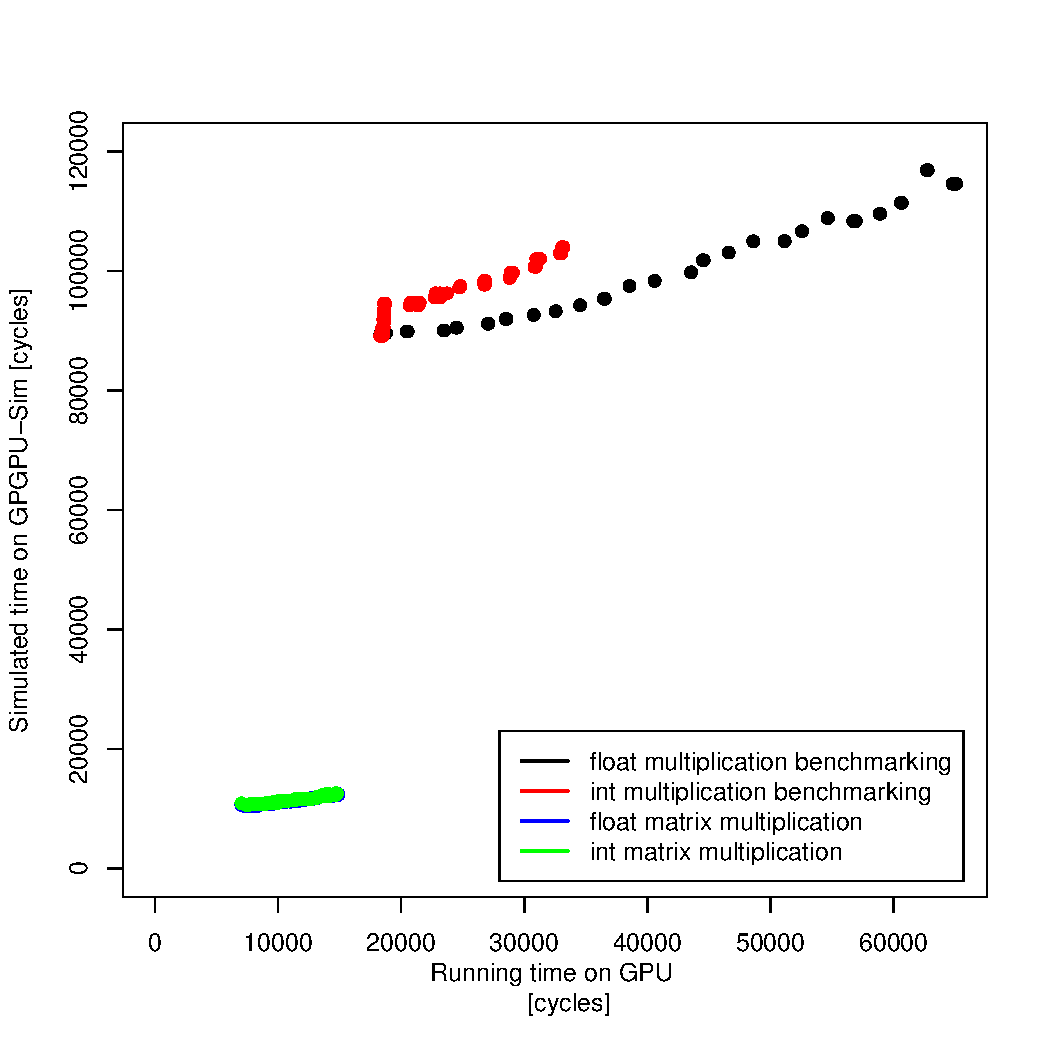
\includegraphics[width=0.7\linewidth]{pictures/comparative_graph}
            \captionsetup{justification=centering}
            \caption{GTX 580 and GPGPU-Sim running times.}
            \label{fig:gpu-sim-corr}
    \end{figure}

        

        And the Pearson's correlations are in Table \ref{tab:gpu-sim-cor}
        \begin{figure}[H]
        \centering
            \begin{tabular}{ | r | c | }
                \hline
                Program type & Running times correlation \\ \hline
                Float multiplication benchmark & 94\% \\
                Integer multiplication benchmark & 98\% \\
                Float matrix multiplication & 98\% \\
                Integer matrix multiplication & 97\% \\
            \end{tabular}
        \captionsetup{justification=centering}
        \caption{Pearson's correlation of GTX580 and GPGPU-Sim running times.}
        \label{tab:gpu-sim-corr}
        \end{figure}

As there is no dependency between the even and odd instructions and there isn't any "new" thread to run, the scheduler looks for the next instruction of the threads belongings to the first two warps.
\begin{figure}[H]
      \centering
       \begin{tabular}{ | r || c | c | c | c || c | c | c | }
    	    \hline
    	    time since beginning & $C_1$ & $C_2$ & ... & $C_{16}$ & $C_{17}$ & ... & $C_{32}$ \\ \hline  \hline
    	   1 & $t_{0,0}$ & $t_{1,0}$ & ... & $t_{15,0}$ & $t_{32, 0}$ & ... & $t_{47, 0}$ \\ \hline 
    	   2 & $t_{16,0}$ & $t_{17,0}$ & ... & $t_{31,0}$ & $t_{48, 0}$ & ... & $t_{63, 0}$ \\ \hline
    	   3 & $t_{0,1}$ & $t_{1,1}$ & ... & $t_{15,1}$ & $t_{32, 1}$ & ... & $t_{47, 1}$ \\ \hline
           4 & $t_{16,1}$ & $t_{17,1}$ & ... & $t_{31,1}$ & $t_{48, 1}$ & ... & $t_{63, 1}$ \\ \hline
    	   5 & - & - & ... & - & - & ... & - \\ \hline
    	   ... & ... & ... & ... & ... & ... & ... & ... \\ \hline
    	   18 & - & - & ... & - & - & ... & - \\ \hline
    	   19 & $t_{0,2}$ & $t_{1,2}$ & ... & $t_{15,2}$ & $t_{32,2}$ & ... & $t_{47,2}$ \\ \hline
    	   ... & ... & ... & ... & ... & ... & ... & ... \\ \hline
  	\end{tabular}
  	\captionsetup{justification=centering}
  	\caption{Planned running scheme for 64 threads with interleaved dependent float multiplication.}
  	\label{fig:fp_prediction_64_halfdep}
   \end{figure}
   
   \bibliography{project_report}{}
   \bibliographystyle{plain}


\end{document}
